\documentclass{article}

\usepackage{geometry}
\geometry{
	a4paper,
	top=13mm,
	left=15mm,
	right=15mm,
	bottom=15mm,
}

\usepackage[document]{ragged2e}
\usepackage[italian]{babel}
\usepackage{graphicx}
\usepackage{multicol}
\usepackage{listings}
\usepackage{color}

\definecolor{dkgreen}{rgb}{0,0.6,0}
\definecolor{gray}{rgb}{0.5,0.5,0.5}
\definecolor{mauve}{rgb}{0.58,0,0.82}

\lstset{frame=tb,
  language=Java,
  aboveskip=3mm,
  belowskip=3mm,
  showstringspaces=false,
  columns=flexible,
  basicstyle={\small\ttfamily},
  numbers=none,
  numberstyle=\tiny\color{gray},
  keywordstyle=\color{blue},
  commentstyle=\color{dkgreen},
  stringstyle=\color{mauve},
  breaklines=true,
  breakatwhitespace=true,
  tabsize=3
}

\graphicspath{{../../immagini/java}}

\begin{document}
Java è un linguaggio di programmazione orientato agli oggetti (OOP), ovvero si manipolano degli oggetti facendogli fare quello che vogliamo.\\
Ciò che un oggetto può fare è scritto nella classe di quell'oggetto.\\
Per installare java sul prorpio pc, serve il java development kit (JDK) che permette di creare e compilare programmi java.\\
Al suo interno troviamo il compilatore, il javadoc e il java run-time environment (JRE).\\
Per compilare un programma java, si usa il comando javac che, eseguito su un file di estensione java (il nostro codice sorgente), restituisce un nuovo file di estensione class (byte code).\\
\textbf{N.B} Il byte code non è un linguaggio direttamente interpretabile dalla macchina (linguaggio macchina/assembly), ma è un linguaggio intermedio.\\
Qui interviene il JRE che contiene l'indispensabile per eseguire codice compilato java.\\
Avremo al suo interno la java virtual machine (JVM), che verrà chiamata in casua dal comando java, avente lo scopo di tradurre il bytecode in linguaggio macchina e di eseguirlo.\\
\textbf{N.B.} Una volta compilato, il byte code può essere eseguito su qualsiasi macchina, basta che ci sia installato java (scrivi una volta, esegui ovunque).\\

\begin{figure}[h]
	\centering
	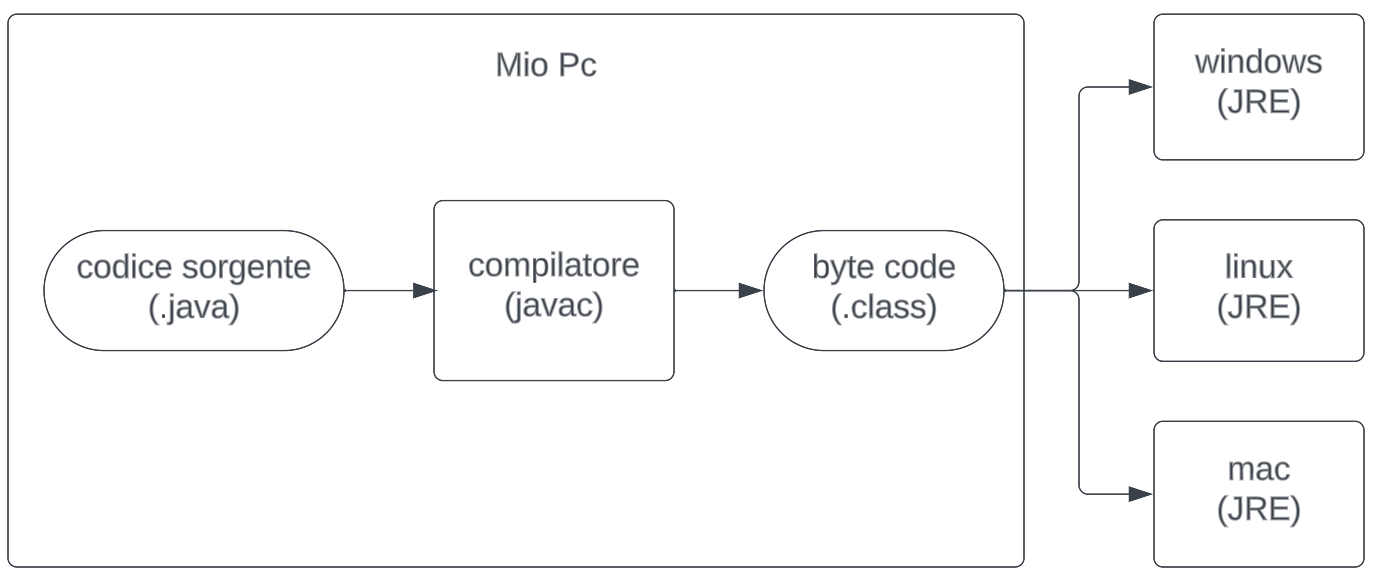
\includegraphics[width=8cm]{processo_esecuzione_java}
\end{figure}

Se, invece del compilatore di default del JDK, ne volesssimo usare un altro, allora avremo bisogna di un integrated development environment (IDE) come eclipse.\\

\section*{Concetti java}

\section*{Classe, Oggetto, Tipo}

Non sono la stessa cosa.
La classe definisce lo scheletro dell'oggetto, ci dice come creare/instanziare l'oggetto, che parametri ha l'oggetto e cosa può fare.\\
L'oggetto, invece, è un entità avente uno stato, un comportamento ed un'identità.\\
Il tipo di un oggetto indica la sua interfaccia (non si riferisce al concetto di interface di java).

\section*{Ereditarietà}

L'ereditarietà in java è un meccanismo di riusco di codice dove un oggetto acquisisce tutte le proprietà e i comportamenti di un oggetto padre.\\
Il riuso tramite sottoclasse è \textbf{white-box} dove i dettagli interni delle superclassi sono spesso visibili alle sottoclassi.\\
L'idea dietro al concetto di ereditarietà in java è che noi possiamo creare una nuova classe costruita sulla base di un'altra classe.\\
Quando si eredita da una classe esistente, possiamo ridefinire i metodi della classe padre (override del metodo), aggiungere nuovi campi e/o metodi.\\
Esistitono due tipi di ereditarietà, che sono legate tra loro, \textbf{ereditarietà di classe} e di \textbf{interfaccia}.\\
La prima l'abbiamo vista prima.\\
La seconda, detta \textbf{subtyping}, dice quando un oggetto può essere usato al posto di un altro oggetto.\\
Al concetto di subtyping è collegato il concetto di \textbf{polimorfismo} e \textbf{binding dinamico}.\\
Polimorfismo è un concetto per il quale un oggetto può assumere più forme, può eseguire la stessa azione in diverse forme.\\
Abbiamo due tipi di polimorfismo, quello a tempo di compilazione e quello a tempo di esecuzione (run-time).\\
Il primo si riferisce al \textbf{method overloading}, ovvero è possibile avere più metodi con lo stesso nome ma con valore in input differenti.\\
Il secondo è il binding dinamico, ovvero ricerca dinamica del metodo, ovvero ricerca a run-time del metodo da chiamare in base al tipo run-time dell’oggetto.\\
Date due classi A e B, tale che $B<:A$, supponiamo che A abbia un metodo m() e supponiamo che B lo ridefinisce.\\
Andiamo nel main, instanziamo un oggetto B e lo salviamo in una variabile di tipo A e chiamiamo su questa variabile il metodo m().\\
La nostra variabile, staticamente (tempo di compilazione), è di tipo A quindi, in teoria, ci aspettiamo di chiamare A.m(), invece, a tempo esecuzione (run-time), il compilatore vede che è di tipo B, quindi chiamerà B.m().\\

\subsection*{Vantaggi}

Definita a tempo di compilazione e controllata staticamente.\\
Facile modificare un’implementazione che si sta riusando tramite method override.\\
Ridefinendo solo alcuni metodi si modifica il comportamento anche degli altri metodi della classe base, se questi chiamano i metodi che stiamo ridefinendo.

\subsection*{Svantaggi}

Definita a tempo di compilazione, la classe parent non può essere cambiata a run-time, i dettagli delle superclassi influiscono molto sulle sottoclassi.\\
Modifiche piccole alle superclassi possono richiedere cambiamenti completi e complessi nelle sottoclassi (fragile base class problem).\\
Le superclassi espongono dettagli alle sottoclassi (inheritance breaks encapsulation).\\
La dipendenza stretta, forte e statica nell’inheritance può creare problemi quando si cerca di riusare una sottoclasse in quanto le superclassi potrebbero non essere appropriate in nuovi contesti, si dovrebbe modificare le superclassi oppure si dovrebbe creare nuove sottoclassi da superclassi differenti.\\
Quindi la dipendenza forte limita la flessibilità e la riusabilità (ciò non accade se si utilizzano calssi astratte).\\

\section*{Riferirsi sempre ad interfacce/classi astratte}

E' buona norma riferirsi sempre ad interfacce o classi astratte nella dichiarazione di un campo e nei tipi usati nelle firme dei metodi.\\
Manipolare oggetti solo in termini di interfacce (o classi astratte) ha due benefici, i client non devono conoscere i tipi specifici degli oggetti, purché aderiscano alle interfacce richieste, non devono conoscere chi implementa tali oggetti (classi concrete) e non dovranno essere modificati se cambiano le implementazioni (classi concrete).\\

\section*{Object composition}

Altro meccanismo di riuso di codice, assemblare più oggetti per creare oggetti più complessi.\\
Il riuso tramite object composition è \textbf{black-box} dove nessun dettaglio interno degli oggetti assemblati è visibile.\\
Gli oggetti sono come scatole nere, accessibili solo tramite le loro interfacce.\\

\subsection*{Vantaggi}

Object composition è definita a run-time e richiede che le interfacce degli oggetti siano rispettate.\\
Gli oggetti sono usati solo tramite le loro interfacce (we don’t break encapsulation).\\
Non si dipende dalle loro implementazioni ma solo dalle loro interfacce e gli oggetti possono essere rimpiazzati tramite subtyping.

\subsection*{Svantaggio}

Il comportamento del programma dipenderà dalla collaborazione di diversi e tanti oggetti, che dovranno essere definiti e assemblati a dovere.

\section*{Astrazione}

Concetto particolare dell'OOP.\\
In java abbiamo due modi per astrarre, usando le classi astratte oppure le interfacce.\\
Con l'astrazione il programmatore decide di mostrare "al mondo" solamente le parti rilevanti dell'oggetto, lasciando il resto nascosto all'utente.\\
Per esempio, quando siamo in auto, sappiamo che se premiamo l'acceleratore, la macchina andrà più forte, altrimenti, se premiamo il freno, la macchina tenderà a rallentare e, alla fine, ad arrestarsi.\\
Però, noi, non sappiamo cosa succede effettivamente quando compiamo queste due azioni, non sappiamo cosa succede dietro.\\
La macchina ci mostra due pedali che sappiamo che fanno due cose differenti, ma non sappiamo il come lo fanno.\\
Una classe si dice astratta quando utilizza la keyword abstract ed ha almeno un metodo astratto, un metodo definito solo dalla sua firma.\\
Sarà compito delle sottoclassi implementare quel metodo, in caso contrario, se non dovessero implementarlo, allora anch'essa diverrebbero astratte.\\
Non è possibile instanziare, direttamente (chiamare il construttore della classe stessa), classi astratte, invece è possibile instanziarla attraverso le sue sottoclassi.\\
Lo scopo della classe astratta è quella di definire una superclasse che definisce la struttura di un oggetto senza provvedere alla sua completa implementazione.\\

\section*{Incapsulamento}

Principio secondo il cui si utilizza una funzione senza sapere cosa fa al suo interno.\\

\end{document}